\documentclass[11pt]{article}
\usepackage[T1]{fontenc}
\usepackage{lmodern,microtype}
\usepackage{amsmath,amssymb,amsthm,mathtools}
\usepackage{booktabs,array,enumitem,tikz}
\usepackage[margin=25mm]{geometry}
\usepackage{xurl}
\usepackage[colorlinks=true,linkcolor=blue!50!black,citecolor=blue!50!black,urlcolor=blue!50!black]{hyperref}
\newcommand{\workbenchurl}{https://github.com/KokunoYumeto/arithmetic-geometry-complexity-workbench}
\newcommand{\recordurl}{https://github.com/KokunoYumeto/mathematics-workbenches}
\newcommand{\AND}{\mathbin{\wedge}}
\newcommand{\OR}{\mathbin{\vee}}
\newcommand{\FG}{F_G}
\newcommand{\supp}{\operatorname{supp}}
\newtheorem{theorem}{Theorem}[section]
\newtheorem{lemma}[theorem]{Lemma}
\newtheorem{corollary}[theorem]{Corollary}
\newtheorem{proposition}[theorem]{Proposition}
\theoremstyle{definition}
\newtheorem{definition}[theorem]{Definition}
\theoremstyle{remark}
\newtheorem{remark}[theorem]{Remark}
\setlist{nosep}
\title{Exact gate counts for theta graphs and cycles with pendant leaves,\\
after jiaxun530 and fengqiaoqu}
\author{}
\date{}
\begin{document}
\maketitle

\begin{abstract}
In the PEqualNP circuit programme, fengqiaoqu proved that a theta graph
without a four-cycle has monotone circuit size equal to its number of edges
plus its vertex-cover number minus one; jiaxun530 used first branching wires
to prove an all-gate lower bound for a particular theta. We show that the
same exact size holds when arbitrary internal NOT gates are allowed and
charged. In particular, the edge function of two seven-cycles sharing an
edge requires eighteen gates. The main lemma states that a graph of minimum
degree at least two without a four-cycle requires at least its number of
vertices plus its cover number minus one binary gates, even in the presence
of negations. We re-prove the positive theta theorem in the form needed for its
equality case, making the argument self-contained for every theta.
We also determine the exact charged-gate size of an even cycle with two
pendant leaves, including fourteen gates for the eight-cycle with leaves
at vertices zero and three. Three nonadjacent leaves on an odd cycle,
separated by odd distances, give another exact formula and seventeen gates
for the nine-cycle with roots zero, three and six.
The mathematics and text were produced by GPT-6 Astra Pro and checked by
separate instances of that model and finite computations; no human has
checked them.
\end{abstract}

\section{The result and its scope}

An exact lower bound must account for sharing as well as for negation.
Let $G=(V,E)$ be a finite simple graph, and write $n=|V|$, $m=|E|$
and $N(v)$ for the neighbors of $v$. Its \emph{edge function} is
\[
  F_G(x)=\bigvee_{\{u,v\}\in E}(x_u\AND x_v),
  \qquad x\in\{0,1\}^{V}.
\]
For a set $S\subseteq V$, write $F_G(S)$ for the value on the input
whose true vertices are precisely $S$. Write $\tau(G)$ for the minimum
size of a vertex cover, a set meeting every edge. A circuit is a finite acyclic straight-line program whose gates are
AND, OR and NOT. AND and OR have fan-in at most two. Every gate, including
NOT, costs one. An input or a gate output can feed arbitrarily many gates.
The minimum total size is denoted by $C(G)$; restricting to AND and OR gives
$C_+(G)$.

The precise straight-line semantics also permit empty input lists, repeated
operands, unused gates and arbitrary natural-number references. Empty AND
is true; empty OR is false. NOT negates its first operand, using false when
it is absent and ignoring a possible second operand. A reference to a wire
not yet available is false. The chosen output is any wire index, with an
out-of-range output again false. These are the semantics of the pinned
\texttt{HasCircuitSize} definition in the PEqualNP project\cite{project}.
Lemma~\ref{lem:normalization} justifies the simpler DAG used in the proof.

\begin{theorem}[Binary gates with arbitrary negations]\label{thm:binary}
Let $G$ be a nonempty finite simple graph on $n$ vertices. Suppose every
vertex has at least two neighbors and $G$ contains no four-cycle, including
a four-cycle with additional chords. Every circuit computing $F_G$ has at
least $n+\tau(G)-1$ binary AND/OR gates. In particular, a normalized such
circuit with $t$ NOT gates has at least $n+\tau(G)-1+t$ gates in total.
\end{theorem}

Here ``binary gates'' in a normalized circuit means exactly two distinct
earlier operands. In an original program, the theorem in particular gives
the same lower bound on the number of listed AND/OR gates; normalization
never introduces an AND/OR gate from a NOT gate.

\begin{theorem}[Theta graphs]\label{thm:theta}
Let $G$ be a simple theta graph: two distinct hubs joined by three distinct paths
with pairwise disjoint interiors, at most one of which is the direct hub edge. If $G$ contains no four-cycle, then
\[
                 C(G)=C_+(G)=|E|+\tau(G)-1.
\]
Every gate is charged, and the conclusion allows arbitrary DAG sharing and
arbitrary internal negations.
\end{theorem}

The monotone equality in this statement is fengqiaoqu's theorem\cite{mono}.
Our argument extends its lower bound to the charged all-gate basis.
It does not assert that every circuit can be made monotone without cost.
Theorem~\ref{thm:binary} leaves exactly one gate between its binary lower
bound and the monotone optimum for a theta. A NOT would itself use that
gate; a circuit without NOT is subject to the monotone lower bound.

\begin{corollary}[Two seven-cycles with a common edge]\label{cor:18}
Let $F$ be the following labelled Boolean function on twelve inputs:
\begin{align*}
F(x)={}&x_0x_1\OR x_0x_2\OR x_2x_3\OR x_3x_4\OR x_4x_5
       \OR x_5x_6\OR x_6x_1\\
     &\OR x_0x_7\OR x_7x_8\OR x_8x_9\OR x_9x_{10}
       \OR x_{10}x_{11}\OR x_{11}x_1,
\end{align*}
where juxtaposition means AND. Its minimum circuit size is eighteen.
Equivalently, in the pinned project semantics,
\[
 \neg\,\texttt{HasCircuitSize}\;12\;F\;17,
 \qquad \texttt{HasCircuitSize}\;12\;F\;18.
\]
\end{corollary}

\begin{theorem}[Two leaves on an even cycle]\label{thm:leaves}
Let $k\ge3$, and attach one fresh pendant leaf to each of two distinct
vertices $a,b$ of the cycle $C_{2k}$. Its two bipartition classes are the
alternating cycle positions. If $G$ is the resulting graph, then
\[
C(G)=
\begin{cases}
3k+1,&a,b\text{ belong to the same bipartition class},\\
3k+2,&a,b\text{ belong to opposite bipartition classes}.
\end{cases}
\]
In particular, for the cycle $0,1,\ldots,7,0$ with additional edges
$08$ and $39$, the exact minimum is fourteen.
\end{theorem}

\begin{theorem}[Three separated leaves on an odd cycle]\label{thm:threeleaves}
Let $k\ge4$. On the cycle $C_{2k+1}$ choose three distinct pairwise
nonadjacent roots, with an odd number of edges in each of the three arcs
between consecutive roots. Attach one fresh pendant leaf to each root.
The resulting graph has exact charged AND/OR/NOT circuit size $3k+5$.
In particular, the nine-cycle with leaves at $0,3,6$ requires seventeen gates.
\end{theorem}

\begin{figure}[ht]
\centering
% Editable labelled graph; created for this workbench.
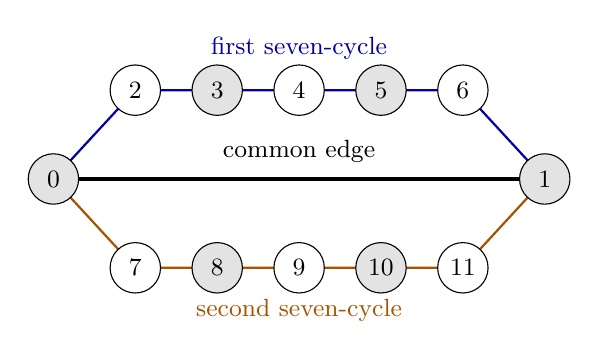
\begin{tikzpicture}[x=1.04cm,y=.94cm,
  vertex/.style={circle,draw=black,fill=white,minimum size=6.4mm,inner sep=1pt},
  chosen/.style={vertex,fill=gray!22},every node/.style={font=\small}]
\coordinate (a) at (0,0); \coordinate (b) at (6,0);
\foreach \i in {1,...,5} {
  \coordinate (p\i) at (\i,1.2);
  \coordinate (q\i) at (\i,-1.2);
}
\draw[very thick] (a)--node[above=2pt] {common edge} (b);
\draw[thick,blue!65!black] (a)--(p1)--(p2)--(p3)--(p4)--(p5)--(b);
\draw[thick,orange!65!black] (a)--(q1)--(q2)--(q3)--(q4)--(q5)--(b);
\node[chosen] at (a) {$0$}; \node[chosen] at (b) {$1$};
\foreach \i/\v in {1/2,3/4,5/6} {\node[vertex] at (p\i) {$\v$};}
\foreach \i/\v in {2/3,4/5} {\node[chosen] at (p\i) {$\v$};}
\foreach \i/\v in {1/7,3/9,5/11} {\node[vertex] at (q\i) {$\v$};}
\foreach \i/\v in {2/8,4/10} {\node[chosen] at (q\i) {$\v$};}
\node[blue!65!black] at (3,1.77) {first seven-cycle};
\node[orange!65!black] at (3,-1.77) {second seven-cycle};
\end{tikzpicture}

\caption{The thirteen-edge graph of Corollary~\ref{cor:18}. Each long path
and the common edge form a seven-cycle. Shaded vertices form the unique
minimum cover $\{0,1,3,5,8,10\}$.}
\label{fig:theta}
\end{figure}

The public circuit programme proposes the lower bound $|E|+\tau(G)-1$ for
all graphs of maximum degree three whose cycles have length at least seven\cite{proposal}. The corollary
settles its explicit adjacent-hub theta. The theorem settles all theta
graphs covered by that proposal, and also some with smaller girth.
The cycle theorems handle specified pendant attachments. Graphs with
arbitrary numbers and arrangements of degree-three vertices remain open.
To state the logical relation explicitly, applying the proposed universal
inequality to this graph gives $13+6\le s+1$, hence $s\ge18$;
Lemma~\ref{lem:parameters} verifies its graph and cover hypotheses.
Conversely, a seventeen-gate circuit here would give $19\le18$ under that
universal statement and would therefore refute it. The proof below settles
this instance directly and does not prove the universal statement.
The result is a finite exact circuit theorem; no conclusion about
P versus NP follows from it.

\paragraph{Credit and neighbouring work.}
The first-branch partition and its one-bit factorization come from
jiaxun530's proof for a different theta\cite{branch}. We write that argument
as a general graph lemma and replace a finite twin-class computation by a
direct vertex-cover construction. The positive-circuit equality analysis
in Section~\ref{sec:positive} follows fengqiaoqu's carrier argument\cite{mono}
and is re-proved here for all theta graphs. The re-proof isolates the
equality case needed both for negations and for pendant leaves, and
writes its cover count explicitly. The historical single-level conjecture
for quadratic Boolean functions concerns a different comparison of monotone
circuits; Jukna's Theorem 2.1\cite{jukna-single} exhibits a linear versus
nearly quadratic gap and shows why an arbitrary
quadratic function cannot simply be assumed to have an optimal star
construction. The hazard derivative of Ikenmeyer, Komarath, Lenzen, Lysikov,
Mokhov and Sreenivasaiah\cite{hazard} compares monotone and hazard-free
complexity. That comparison does not exclude circuits with hazards.
Jukna's later syntactic transformation\cite[Theorem 1]{jukna-hazard}
also requires absence of hazards. The communication game of Ikenmeyer,
Komarath and Saurabh\cite[Theorem 4.6]{hazard-games} characterizes hazard-free
formula size and depth. Here the cut argument controls shared circuit DAGs
with arbitrary hazards.
OpenAI's First Proof submissions\cite{openai} report model-written arguments
and subsequent expert feedback, providing recent methodological context for
the separate mathematical and formal verification statuses at the end.

\section{Proof overview}

The difficulty is that a negation can affect many later gates through shared
wires, so local elimination must not silently replace the original circuit
by a formula. Instead, follow each input until its first branching wire,
or until the output if no branch is reached. All influence of that input
passes through this terminal wire. Inputs with the same terminal form a
group.

Two adjacent graph vertices cannot belong to one group. With all other
inputs zero their restriction is AND; with suitable independent neighbors
on, it is OR. At the common terminal, each variable occurs only once in
an unfolded formula. A read-once pair cannot change between those two
functions by changing exterior values and applying one final unary map.
Minimum degree supplies the neighbors; the absence of a four-cycle ensures
that they are independent.

Order the groups by their terminal wires. After earlier groups are removed,
the active vertices in the next group have identical neighborhoods among
later groups: the circuit communicates the selected vertices of that group
through only one bit. In a graph without a four-cycle, such a twin group
meets its remaining edges in a star. Choose the center of that star. These
chosen centers form a vertex cover, using at most one vertex per branch.
Hence there are at least $\tau(G)$ branching wires. Counting operand
incidences then gives $n+\tau(G)-1$ binary gates, with every NOT charged in
addition. For the displayed theta, this is seventeen binary gates. A
seventeen-gate circuit would therefore be positive, and its positive
lower bound is eighteen.

For a positive circuit at the binary lower bound, singleton inputs identify
exactly one branching carrier for each vertex of a minimum cover. Each
carrier has only two exits, so it can lose its singleton value at at most
two gates. Every edge to an unselected neighbor needs its own such gate;
selected neighbors need at least one more. Summing these requirements
contradicts the fact that a theta has one more edge than vertex, while a
minimum cover induces a forest. This gives the full positive theta bound.
For a cycle with leaves, setting the leaves to zero preserves a lower bound
on branches. At equality the selected cycle vertices form one alternating
class, and a selected attachment root would need three consumption gates.
The parity of two roots decides whether this obstruction occurs. On an
odd cycle with three separated roots, the unique edge inside a minimum
cycle cover cannot accommodate all roots that would need an extra exit.

\section{Normalizing and counting a circuit}

This section proves that the unusual legal programs in the project do not
escape the DAG argument.

\begin{lemma}[Normalization]\label{lem:normalization}
For a nonconstant function which is not a primary input, every legal program
can be replaced, without increasing either its AND/OR count or its NOT
count, by one with valid earlier references, binary AND/OR gates with
distinct operands, unary NOT gates, final output, and no gate outside the
output's ancestor cone. If every input is essential, every nonoutput wire
has a consumer. In a least circuit, a semantically constant gate or a gate
equal to an earlier wire can also be excluded.
\end{lemma}
\begin{proof}
Process the original gates in order. Maintain a map sending each original
wire to a static Boolean value or to an earlier wire of the new program.
An unavailable read maps to false at the step when it is read. Discard any
second NOT operand. Evaluate constant operations and apply
$0\AND z=0$, $1\AND z=z$, $0\OR z=z$, $1\OR z=1$.
Unary AND/OR and repeated-operand binary gates are copies. Every remaining
gate has precisely the claimed form. Each old gate produces zero new gates
or one new gate of the same operation. Induction over the original list
proves preservation of every mapped value and of the selected output.

The new output cannot be static or a primary input by the hypotheses.
Delete gates outside its ancestor cone and renumber the remaining gates in
their old order. Any gate after the output is outside that cone, so the
output is last. Every remaining gate reaches it. An essential input must
also reach it, since otherwise changing that input could not affect the
output. Finally, a semantically constant or copy-valued gate in a least
circuit could be substituted and eliminated by the same construction,
contradicting leastness.
\end{proof}

For an edge function with no isolated vertices every input is essential:
if $uv$ is an edge, the supports $\{u\}$ and $\{u,v\}$ give different
outputs. The function is nonconstant and false at every singleton, so it
is not a primary input.

Orient circuit edges from operands towards consuming gates. A
\emph{branching wire} has at least two distinct consumers. Distinct binary
operands make this an ordinary DAG without duplicated arcs.

\begin{lemma}[Incidence budget]\label{lem:budget}
A normalized circuit with $n$ essential inputs, $g$ gates, $t$ NOT gates
and $b$ branching wires satisfies
\[
                  g\ge n-1+b+t.
\]
If equality holds, every branching wire has exactly two consumers and
every other nonoutput wire exactly one.
\end{lemma}
\begin{proof}
There are $n+g$ wires. Every wire except the output has a consumer, and each
branching wire contributes at least one additional operand incidence.
There are therefore at least $n+g-1+b$ incidences. Counting at the gates
gives $2(g-t)+t=2g-t$ incidences. Rearranging proves the inequality.
Equality forces equality in each outdegree bound.
\end{proof}

\section{First branches give a vertex cover}

We now prove the structural part of Theorem~\ref{thm:binary} for the same
original normalized DAG throughout.

\begin{definition}
Starting from a primary input $v$, follow its unique consumer until reaching
a branching wire or the output. The first such wire is its
\emph{terminal} $r(v)$. The inputs with the same terminal form its
\emph{terminal group}.
\end{definition}

The path terminates because the circuit is finite and acyclic. Before
$r(v)$ it has no choice. Thus every path from $v$ to the output passes
through $r(v)$, and there is exactly one path from $v$ to $r(v)$.
When the expression at $r(v)$ is unfolded into a formula, $v$ occurs
exactly once. This use of a local unfolding does not replace the circuit
or change its gate count.

We use the following cut principle repeatedly. If every path from a set
of primary inputs to the output meets a wire $c$, then two assignments
which agree outside that set and have the same value at $c$ have the same
output. To prove it, regard $c$ as a new primary and delete its incoming
arcs. No path from a changed primary to the output remains. Topological
induction shows that each wire reaching the output has the same value on
the two assignments.

\begin{lemma}[A read-once pair]\label{lem:pair}
Let a formula over AND, OR and NOT contain each of two variables $a,b$
at most once. Among restrictions of its other variables which leave it
dependent on both $a,b$, its resulting two-variable function is fixed.
\end{lemma}
\begin{proof}
Push negations to leaves by De Morgan's laws; this changes no occurrence
count. If both variables occur, take the least common ancestor of their
two signed leaves. Every attached subtree on the two paths up to this
ancestor contains neither variable, and is constant after restriction.
To preserve both dependencies it must take the neutral value of its
parent AND or OR gate. The same is true on the path from this ancestor
to the formula output. The resulting function is the fixed operation at
the ancestor applied to the two fixed signed literals. If a variable was
absent, a restriction depending on both cannot occur.
\end{proof}

\begin{lemma}[Independent groups]\label{lem:independent}
If $G$ has minimum degree at least two and no four-cycle, every terminal
group of a circuit for $F_G$, including the output group, is independent
in $G$.
\end{lemma}
\begin{proof}
Suppose adjacent vertices $i,j$ have common terminal $r$. Each occurs once
in a formula unfolded at $r$. All their influence on the output passes
through $r$, so with exterior inputs fixed the output is a unary function
of that formula's value.

Choose neighbors $u$ of $i$ and $v$ of $j$ with $u\ne j$ and $v\ne i$.
They lie outside $\{i,j\}$. They are nonadjacent: if equal, simplicity
gives this; if distinct, an edge $uv$ would give the four-cycle
$i,j,v,u,i$. With all exterior inputs zero, the output on $i,j$ is
$i\AND j$. With just $u,v$ on outside $\{i,j\}$, it is $i\OR j$.
In each case the value at $r$ depends on both variables and the subsequent
unary map is nonconstant. Lemma~\ref{lem:pair} gives the same function at
$r$ in both cases. The two nonconstant unary Boolean maps are identity
and complement. But AND and OR are neither equal nor complementary.
This contradiction proves the lemma.
\end{proof}

\begin{lemma}[Residual twins]\label{lem:twins}
Order the branching terminals by their circuit indices, with the output
last. Delete all terminal groups earlier than a branching terminal $r$.
Among the vertices of its group which still have a neighbor, all remaining
neighborhoods are equal.
\end{lemma}
\begin{proof}
Let $Q$ be the group of $r$, and let $R$ consist of the vertices in later
groups. By Lemma~\ref{lem:independent}, any remaining neighbor of a member
of $Q$ lies in $R$.
No input in $R$ can reach $r$ in the circuit: along any such path its
first branching wire would occur at or before $r$, whereas its terminal
has larger index. Set all earlier-group inputs to zero. For $S\subseteq Q$
and $T\subseteq R$, turn on precisely $S\cup T$. The value at $r$ depends
only on $S$; call it $c(S)\in\{0,1\}$. By the cut principle the output is
a function $d(c(S),T)$. This factorization requires no monotonicity of
$c$ or $d$.

If $u\in Q$ has a remaining neighbor $w\in R$, then
$F_G(\{u,w\})=1$ and $F_G(\{w\})=0$. Hence
$c(\{u\})\ne c(\varnothing)$. Since the code has only two values,
all such active vertices have the same singleton code. For any $z\in R$,
$uz$ is an edge precisely when $d(c(\{u\}),\{z\})=1$.
Thus their neighborhoods in $R$ coincide.
\end{proof}

\begin{lemma}[One cover vertex per group]\label{lem:cover}
Let a four-cycle-free graph have an ordered partition into independent
groups, with the active vertices of each group having identical
neighborhoods in later groups. If there are $b$ groups before the last,
then $\tau(G)\le b$.
\end{lemma}
\begin{proof}
For each group except the last, consider its edges to later groups.
If none exist, choose nothing. If just one vertex of the group is active,
choose that vertex. Otherwise choose two distinct active vertices. Their
common neighborhood in later groups is nonempty and has at most one
vertex: two distinct common neighbors would form a four-cycle, because
the group and the later groups are disjoint. Choose this unique common
neighbor. In all cases at most one chosen vertex meets every edge from
the group to later groups.

The set of all chosen vertices is a cover. Indeed every edge has endpoints
in different groups, and is covered when its earlier group is considered.
There are no edges wholly inside the last group. Repeated choices only
decrease the size of the resulting cover.
\end{proof}

For example, in a three-vertex path the two end vertices are a twin group;
choosing their common middle neighbor covers both remaining edges. This
is why one cannot merely assume every group is a singleton. The absence
of a four-cycle says that every larger active twin group has exactly this
star form.

\begin{proof}[Proof of Theorem~\ref{thm:binary}]
Normalize the circuit using Lemma~\ref{lem:normalization}. Its terminal
groups are independent by Lemma~\ref{lem:independent} and satisfy the
residual-twin condition by Lemma~\ref{lem:twins}. Add empty groups at
branching wires with no labelled primary if needed. There are at most
$b$ groups before the output, where $b$ is the number of branching wires.
Lemma~\ref{lem:cover} gives $b\ge\tau(G)$. The incidence budget gives
$g-t\ge n-1+b\ge n+\tau(G)-1$. Normalization does not increase the
AND/OR count, so the same count lower bound holds for the original program.
\end{proof}

\section{The positive theta bound}\label{sec:positive}

This section re-proves fengqiaoqu's monotone theta theorem\cite{mono} in
a form that exposes its equality obstruction. The local carrier argument
also applies to vertices of degree at least two in graphs with leaves.

In a normalized positive circuit every wire is zero on the all-zero input.
A wire \emph{carries} $v$ if it is one on the singleton input $\{v\}$.
Its \emph{singleton support} is the set of vertices it carries.
Every carrier of $v$ is reached by a path of carriers from the primary $v$:
trace backwards through a true parent of an OR, or either parent of a true
AND. Call $v$ \emph{eligible} if some carrier of $v$ branches. For an
eligible $v$, let $b(v)$ be its earliest branching carrier. Its carrier path
from $v$ has unique exits before $b(v)$, so $b(v)$ cuts all influence of $v$.
If $v$ is ineligible, the same is true of every carrier of $v$.

\begin{lemma}[Carrier facts]\label{lem:carrier}
Let $G$ have no four-cycle, and consider a normalized positive circuit
for its edge function. The eligible vertices meet every edge whose two endpoints have
degree at least two. If $v$ has degree at least two, a carrier of $v$
which cuts all influence of $v$ carries no other vertex. Consequently
distinct eligible vertices of degree at least two have distinct first
branching carriers. If every vertex has degree at least two, the eligible
set is a vertex cover.
\end{lemma}
\begin{proof}
For an edge $uv$ whose endpoints have degree at least two, take the first
wire which is one on $\{u,v\}$ and zero
on both singletons. It is an AND gate, since otherwise a parent of an OR
would be an earlier such wire. Its parents can be labelled $a,b$ so that
$a$ carries $u$ but not $v$, and $b$ carries $v$ but not $u$: both are one
on the pair; by firstness each carries an endpoint; and neither singleton
makes both parents true. Call this a meeting gate for $uv$.

If both endpoints were ineligible, their carrier routes to these parents
would have unique exits leading to the meeting gate. That gate would cut
all influence of $u,v$; moreover $a$ would not depend on $v$, nor $b$ on
$u$. Choose alternate independent neighbors as in
Lemma~\ref{lem:independent} and switch them on. The output is initially
zero, and becomes one after either endpoint alone is turned on. The cut
principle and positivity force the meeting gate to change from zero to
one in each case. The change of $u$ cannot affect $b$, so $b$ was already
one; similarly $a$ was already one. Their AND was therefore already one,
a contradiction. The eligible set meets every such edge.

For the second claim, suppose a cut carrier $c$ of $v$ also carries
$w\ne v$. There is a neighbor $z$ of $v$ nonadjacent to $w$. If $w$ is a
neighbor of $v$, choose $z=w$. Otherwise, if every neighbor of $v$ were
adjacent to $w$, two distinct such neighbors would give a four-cycle.
The support $\{w,z\}$ is independent. Positivity makes $c$ one both there
and on $\{v,w,z\}$, although the output changes because $vz$ is an edge.
This contradicts the cut principle. Applying this to $b(v)$ proves
injectivity.
\end{proof}

\begin{lemma}[Two consumption exits]\label{lem:slots}
Let $G$ have minimum degree at least two and no four-cycle. Suppose a
normalized positive circuit for $F_G$ has $n+\tau(G)-1$ gates. Its eligible
set $S$ is a minimum cover, its branching wires are precisely $b(v)$ for
$v\in S$, and each has exactly two consumers and singleton support
$\{v\}$. Moreover every $v\in S$ satisfies
\begin{equation}\label{eq:slots}
 |N(v)\setminus S|+\mathbf 1_{N(v)\cap S\ne\varnothing}\le2.
\end{equation}
\end{lemma}
\begin{proof}
Lemma~\ref{lem:carrier} and the incidence budget give
\[
 g\ge n-1+b\ge n-1+|S|\ge n-1+\tau(G).
\]
The assumed gate count forces equality throughout. Hence $S$ is a minimum
cover, its distinct first branching carriers exhaust all branches, and
those branches have exactly two consumers. Their singleton supports follow
from Lemma~\ref{lem:carrier}.

Say a gate \emph{consumes} $v$ if a parent carries $v$ but the gate does not.
Every such gate is reached by a carrier path from $v$. For $v\in S$ that
path passes $b(v)$: before it, the carrier route has only one exit, so
cannot both lose the carrier value and continue to $b(v)$. After $b(v)$,
a $v$-carrier cannot branch again, because every branch is a distinct
$b(w)$ with singleton support $\{w\}$. The two exits of $b(v)$ therefore
allow at most two consumption gates. Merging paths can only reduce this
number. This conclusion uses only the stated structure of the branches,
not the minimum-degree assumption on every vertex of $G$.

Each graph neighbor $u$ of $v$ has a meeting AND gate which consumes $v$.
If two distinct neighbors $u,w$ use the same meeting gate, its unique
parent not carrying $v$ must carry both $u,w$. If either neighbor is
ineligible and has degree at least two, every carrier of that neighbor
is a cut carrier, and Lemma~\ref{lem:carrier} forbids this.
Take all neighbors outside $S$, and one neighbor inside $S$ if any exists.
Any two in this list include an ineligible vertex, so their meeting gates
are distinct. At most two such gates exist, proving~\eqref{eq:slots}.
\end{proof}

\begin{lemma}[Minimum theta covers]\label{lem:thetacovers}
Let a simple theta have $p,q,r$ interior vertices on its three paths.
Set $t=\lfloor p/2\rfloor+\lfloor q/2\rfloor+\lfloor r/2\rfloor$,
and let $o$ be the number of odd parameters. Then
\[
 \tau(G)=t+\min(2,1+o),\qquad 2\tau(G)\le |V|+1=|E|.
\]
Every minimum vertex cover induces a forest.
\end{lemma}
\begin{proof}
There are $n=p+q+r+2=2t+o+2$ vertices and $m=n+1$ edges.
A path on $d$ vertices has cover number $\lfloor d/2\rfloor$: alternating
edges give that many disjoint edges and alternating vertices give a cover.
If both hubs are selected, the three remaining interior paths therefore
cost $t$ additional vertices, for a total $2+t$.

If exactly one hub is selected, the last interior vertex beside the omitted
hub must be selected on each path with $d\ge1$ interiors. Removing it
leaves a path on $d-1$ vertices, so the interior cost is
$1+\lfloor(d-1)/2\rfloor=\lceil d/2\rceil$. A direct hub edge costs no
interior vertex. The total is $1+t+o$.
If neither hub is selected, a direct edge makes a cover impossible.
Otherwise each path's two end interior vertices must be selected. For
$d=1$ this costs one; for $d\ge2$ it costs
$2+\lfloor(d-2)/2\rfloor=1+\lfloor d/2\rfloor$.
Thus this case costs $3+t$ and is never better. Taking the minimum proves
the formula. If $o=0$, then $2\tau=2t+2\le n+1$; if $o\ge1$, then
$2\tau=2t+4\le2t+o+3=n+1$.

Every vertex in a minimum cover $S$ has a neighbor outside $S$, since
otherwise removing it would still leave a cover. Any cycle in a theta
contains an interior vertex, which has degree two in the whole graph.
A cycle inside $G[S]$ would put both its neighbors in $S$, contradicting
that necessary outside neighbor. Therefore $G[S]$ is a forest.
\end{proof}

\begin{proposition}[Positive theta size]\label{prop:positive}
A simple theta without a four-cycle has positive circuit size
$C_+(G)=|V|+\tau(G)=|E|+\tau(G)-1$.
\end{proposition}
\begin{proof}
The incidence budget and Lemma~\ref{lem:carrier} give
$C_+(G)\ge n+\tau(G)-1$. Suppose equality holds and let $S$ be the minimum
cover from Lemma~\ref{lem:slots}. Let $I$ be the edge set of $G[S]$, let
$A$ be its nonisolated vertices, and let $Q$ count edges crossing from $S$
to its complement. Because $S$ is a cover, $m=Q+|I|$. Summing
\eqref{eq:slots} over $S$ gives
\[
                         Q+|A|\le2|S|.
\]
If $I$ is nonempty, the forest in Lemma~\ref{lem:thetacovers} has fewer
edges than nonisolated vertices. Hence
\[
 m=Q+|I|<Q+|A|\le2|S|=2\tau(G)\le m,
\]
a contradiction. If $I$ is empty, $S$ is independent as well as a cover,
so its complement is also a cover. Minimality gives $2|S|\le n$.
The same slot sum gives $m=Q\le2|S|\le n$, contradicting $m=n+1$.
Thus $C_+(G)\ge n+\tau(G)$.

For the upper bound, assign each edge to one selected endpoint in a minimum
cover $S$. Each selected vertex has a neighbor outside $S$, so it receives
at least one edge. If it receives $d$ edges, OR their other endpoints and
AND the result with this vertex, using $(d-1)+1=d$ gates. The resulting
stars partition the edge terms. OR their outputs using $|S|-1$ gates.
The total is $m+\tau(G)-1=n+\tau(G)$, as required.
\end{proof}

\begin{proof}[Proof of Theorem~\ref{thm:theta}]
A simple theta has minimum degree two and $|E|=|V|+1$. Put $n=|V|$ and
$k=\tau(G)$. Proposition~\ref{prop:positive} gives $C_+(G)=n+k$.
Theorem~\ref{thm:binary} requires at least $n+k-1$ AND/OR gates.
A circuit with total size at most $n+k-1$ would normalize to one with no
NOT gates, contradicting the positive lower bound. Thus $C(G)\ge n+k$,
and the positive construction supplies the reverse inequality.
The no-four-cycle condition means exactly that no pair of the three
interior parameters has sum two; a simple theta has at most one zero
parameter. These include the adjacent-hub and triangular cases.
\end{proof}

\section{An explicit eighteen-gate circuit}

We now apply the general theorem to the labelled graph and give its full
numbered circuit.

\begin{lemma}[The labelled graph]\label{lem:parameters}
The graph of Corollary~\ref{cor:18} has twelve vertices, thirteen edges,
minimum degree two, and simple cycles of lengths seven, seven and twelve.
Its unique minimum cover is $S_0=\{0,1,3,5,8,10\}$, of size six.
\end{lemma}
\begin{proof}
The three internally disjoint hub-to-hub paths have lengths one, six and
six. Every simple cycle uses two of them, giving the stated lengths.
The hubs have degree three and all other vertices degree two.
The six pairwise disjoint edges
\[
 (0,2),\ (3,4),\ (5,6),\ (7,8),\ (9,10),\ (11,1)
\]
force every cover to have size at least six, and $S_0$ is a cover.
A cover omitting one hub must include the other. On each long path the
six-vertex segment from its first interior to the omitted hub has a
matching of size three. Since that hub is omitted, at least three interior
vertices on each path must be selected, giving at least seven vertices
altogether. Thus every size-six cover contains both hubs. Each remaining
five-vertex interior path has unique minimum cover at its second and fourth
vertices, proving uniqueness.
\end{proof}

Here the positive obstruction can be seen at one hub: the three neighbors
$1,2,7$ of $0\in S_0$ include two outside $S_0$ and one inside it. They
would require three consumption gates, whereas Lemma~\ref{lem:slots}
allows two at a hypothetical seventeen-gate circuit.

The upper bound follows directly from six stars and is independently
checkable without any lower-bound argument. Define
\begin{align*}
A_0&=x_0\AND(x_1\OR x_2\OR x_7),&
A_1&=x_1\AND(x_6\OR x_{11}),\\
A_3&=x_3\AND(x_2\OR x_4),&
A_5&=x_5\AND(x_4\OR x_6),\\
A_8&=x_8\AND(x_7\OR x_9),&
A_{10}&=x_{10}\AND(x_9\OR x_{11}).
\end{align*}
Distributivity shows that their disjunction is precisely the thirteen
labelled edge terms. The first star costs three gates; each other star
costs two. Five further OR gates combine the stars. The total is
$3+5\cdot2+5=18$.

For a fully indexed witness, primary wires are $0,\ldots,11$ and each row
below defines the indicated new wire. The output is wire $29$.
\begin{center}
\begin{tabular}{rl@{\qquad}rl@{\qquad}rl}
\toprule
Wire&Operation&Wire&Operation&Wire&Operation\\
\midrule
12&$1\OR2$&13&$12\OR7$&14&$0\AND13$\\
15&$6\OR11$&16&$1\AND15$&17&$2\OR4$\\
18&$3\AND17$&19&$4\OR6$&20&$5\AND19$\\
21&$7\OR9$&22&$8\AND21$&23&$9\OR11$\\
24&$10\AND23$&25&$14\OR16$&26&$18\OR20$\\
27&$22\OR24$&28&$25\OR26$&29&$28\OR27$\\
\bottomrule
\end{tabular}
\end{center}

\begin{proof}[Proof of Corollary~\ref{cor:18}]
Lemma~\ref{lem:parameters} and Theorem~\ref{thm:binary} require seventeen
AND/OR gates. A circuit with at most seventeen total gates would normalize
to a positive circuit of at most that size, contradicting
Proposition~\ref{prop:positive}. The explicit circuit proves the upper
bound.
\end{proof}

\section{A cycle with two pendant leaves}\label{sec:leaves}

This section proves Theorem~\ref{thm:leaves}, using the same branch count
and the equality case of the positive argument.

\begin{lemma}[Restriction does not create branches]\label{lem:restriction}
Fix some inputs of a normalized circuit to constants. Propagate constants,
suppress resulting projections and repeated-operand gates, and remove
dead gates. If the resulting function is nonconstant, its normalized
circuit has no more branching wires than the original.
\end{lemma}
\begin{proof}
Deleting a constant wire or a dead gate removes vertices and arcs and
cannot increase an outdegree. The only other graph operation suppresses
a gate $q$ whose remaining value is its single parent $p$. Redirect all
uses of $q$ to $p$, including the selected output if necessary. Write
$d$ for the number of consumers of $p$ other than $q$, and $t$ for the
number of consumers of $q$. The new outdegree of $p$ is at most $d+t$;
coincident uses may reduce it. If neither $p$ nor $q$ previously branched,
then $d=0$ and $t\le1$, so the merged wire does not branch. Otherwise the
one merged wire contributes at most the previous two branch indicators.
All other outdegrees are unchanged or decrease. These operations implement
the local normalization after restriction, proving the claim by induction
on their number. Arbitrary resynthesis of the restricted function is not
part of the operation asserted here.
\end{proof}

\begin{corollary}[An induced core]\label{cor:core}
Let $G$ have $n$ vertices and no isolated vertex. Suppose an induced
subgraph $H$ is nonempty, has minimum degree at least two, and has no
four-cycle. Then
every circuit for $F_G$ has at least $n-1+\tau(H)$ AND/OR gates.
\end{corollary}
\begin{proof}
Normalize the circuit for $G$. Set every input outside $H$ to zero and
use the local simplification of Lemma~\ref{lem:restriction}. The remaining
function is exactly $F_H$. The proof of Theorem~\ref{thm:binary} requires
at least $\tau(H)$ branches in that circuit, so at least as many were
present in the original normalized DAG. Apply Lemma~\ref{lem:budget}
there, with all $n$ original inputs essential.
\end{proof}

\begin{proof}[Proof of Theorem~\ref{thm:leaves}]
The graph has $n=2k+2$ vertices and $2k+2$ edges. Its induced cycle has
cover number $k$. Thus every normalized circuit satisfies
\begin{equation}\label{eq:leafbudget}
                   g\ge3k+1+t,
\end{equation}
where $t$ counts NOT gates.

The only covers of the cycle of size $k$ are its two alternating
bipartition classes. Indeed its complement would be an independent set
of size $k$; around the cycle every gap between consecutive selected
vertices must have exactly one omitted vertex. If the two roots have
the same parity, that class covers the enlarged graph, so $\tau(G)=k$.
If they have opposite parity, no cover of the enlarged graph has size
$k$: its cycle part must already have size $k$, leaving neither leaf
available, and would therefore need both roots. One alternating cover
together with the other root is a cover of size $k+1$.

For completeness, the cover construction assigns each edge to one of
its endpoints in a minimum cover $S$. Every $v\in S$ has a neighbor
outside $S$, since otherwise it could be removed from $S$, so it receives
at least one edge regardless of how edges within $S$ are assigned.
A star with $d$ assigned edges costs $d$ gates: $d-1$ OR gates on its
neighbors and one AND with its center. Joining the $|S|$ stars uses
$|S|-1$ further gates, for a total $|E|+|S|-1$.
This gives upper bounds $3k+1$ and $3k+2$ in the two cases.
Equation~\eqref{eq:leafbudget} settles the same-parity case.

Now suppose the roots have opposite parity, and normalize a circuit of
at most $3k+1$ gates. Equation~\eqref{eq:leafbudget} forces exactly
$3k+1$ gates and $t=0$, so this normalized circuit is positive.
Let $S$ be the eligible \emph{cycle} vertices. Every cycle edge has
endpoints of degree at least two. Lemma~\ref{lem:carrier} therefore
shows that $S$ covers the cycle, and that its first branching carriers
are distinct with singleton supports. There are at least $k$ of them.
Equality in the incidence budget permits only $k$ branches altogether.
Consequently $|S|=k$, $S$ is one alternating class, and these are all the
branches. Each has exactly two consumers. No leaf is eligible, because
each branch carries only its selected cycle vertex.

Exactly one root belongs to $S$; call it $v$. As in the proof of
Lemma~\ref{lem:slots}, only the two exits of $b(v)$ can
lead to gates consuming $v$, so at most two gates consume it. Its three
incident edges each have a meeting AND gate consuming $v$.
The meeting gate exists for any edge, including a leaf edge: take the
first wire true on that pair and false on both singletons, as in the
first paragraph of the proof of Lemma~\ref{lem:carrier}.
These three gates are distinct. If two coincided, their parent not
carrying $v$ would carry both other endpoints. Among any two of the
three neighbors, at least one is an ineligible cycle vertex. Every
carrier of that vertex is a cut carrier, so Lemma~\ref{lem:carrier}
makes its support a singleton, a contradiction. Thus three gates
consume $v$, which is impossible. The opposite-parity case requires
$3k+2$ gates.
\end{proof}

The eight-cycle in Theorem~\ref{thm:leaves} uses opposite classes: vertices $0$ and $3$
have different parity and are not adjacent. An explicit fourteen-gate
witness, returning wire $23$ from primary wires $0,\ldots,9$, is
\begin{center}
\begin{minipage}{0.9\linewidth}
\centering
\begin{tabular}{rl@{\qquad}rl}
\toprule
Wire&Operation&Wire&Operation\\
\midrule
10&$1\OR7$&11&$10\OR8$\\
12&$0\AND11$&13&$1\OR3$\\
14&$2\AND13$&15&$4\OR9$\\
16&$3\AND15$&17&$4\OR6$\\
18&$5\AND17$&19&$6\AND7$\\
20&$12\OR14$&21&$16\OR18$\\
22&$20\OR21$&23&$22\OR19$\\
\bottomrule
\end{tabular}
\end{minipage}
\end{center}
Its five stars have centers $0,2,3,5,7$ and partition the ten edge terms.
Thus distributivity proves correctness and the listed rows establish the
gate count directly.

\section{Three separated leaves on an odd cycle}\label{sec:threeleaves}

The same equality obstruction resolves the next marking with three roots.
We prove Theorem~\ref{thm:threeleaves} by locating a selected root whose two
cycle neighbors are unselected.

\begin{proof}[Proof of Theorem~\ref{thm:threeleaves}]
Write the three cyclic distances as $d_1,d_2,d_3$. By assumption they are
odd and at least three, and $d_1+d_2+d_3=2k+1$. A minimum cover of $G$
can be chosen to contain all three roots and none of the leaves: replace
any selected leaf whose root is absent by that root, and discard any leaf
whose root is present. Once the roots are selected, the three uncovered
interior paths have $d_i-1$ vertices each. Consequently
\[
 \tau(G)=3+\sum_{i=1}^{3}\frac{d_i-1}{2}=k+2.
\]
There are $n=m=2k+4$ vertices and edges. The star construction in the proof of
Proposition~\ref{prop:positive} gives the upper bound
$m+\tau(G)-1=3k+5$.

The induced cycle has cover number $k+1$. Corollary~\ref{cor:core} therefore
requires $n-1+(k+1)=3k+4$ AND/OR gates. Suppose a circuit has at most this
many total gates, and normalize it. It is positive. The restriction
argument in Corollary~\ref{cor:core} requires at least $k+1$ branches;
the incidence budget now forces exactly that many, each with two consumers. As in the two-leaf proof,
the eligible cycle vertices form a cover $S$ of the cycle and have distinct
first branching carriers with singleton supports. Thus $|S|=k+1$, all
branches are those carriers, and no leaf is eligible.

A minimum cover of an odd cycle has exactly one edge with both endpoints
in $S$. Indeed its complement has $k$ independent vertices. Between
consecutive complementary vertices there are $k$ nonempty strings of
selected vertices containing $k+1$ vertices altogether. Exactly one string
has length two and every other has length one. Denote the unique edge
inside $S$ by $e$.

If a marked root $v\in S$ is not an endpoint of $e$, both its cycle
neighbors are ineligible. Its two cycle edges and its leaf edge then have
three distinct meeting gates consuming $v$: any pair of the other endpoints
includes an ineligible cycle vertex, whose cut carriers have singleton
support by Lemma~\ref{lem:carrier}. But the two exits of $b(v)$ allow at
most two such gates, as proved in Lemma~\ref{lem:slots}. Hence every marked
root in $S$ must be an endpoint of $e$. The roots are pairwise nonadjacent,
so at most one belongs to $S$.

At least one root must belong to $S$. If all three were outside, the path
between two consecutive roots would have $d_i-1$ even interior vertices
and both endpoints unselected. Its interior cover would cost
$1+(d_i-1)/2$. Summing over the three disjoint interiors gives at least
$k+2$ selected vertices, contradicting $|S|=k+1$.
Thus exactly one root $v$ lies in $S$ and is an endpoint of $e$.
The arc between the other two roots which does not pass through $v$ has
odd length and has unselected endpoints. It must contain an edge with both
endpoints selected: otherwise, since no edge can have both endpoints
unselected, selection would alternate along this odd arc and its endpoint
selections would differ. Its selected edge cannot be $e$, which is incident
to $v$ outside the arc. This contradicts uniqueness of $e$.
Therefore $3k+4$ gates are impossible, proving the claimed optimum.
\end{proof}

For the nine-cycle, the three distances are $3,3,3$ and $k=4$, so the
optimum is seventeen. One cover construction uses centers
$0,2,3,5,6,8$. With fresh leaves $9,10,11$ at $0,3,6$, respectively,
the six terms are
\[
 x_0(x_1\OR x_8\OR x_9),\quad x_2(x_1\OR x_3),\quad
 x_3(x_4\OR x_{10}),\quad x_5(x_4\OR x_6),\quad
 x_6(x_7\OR x_{11}),\quad x_7x_8.
\]
The first term costs three gates, the last costs one, and each other term
costs two. Their disjunction uses five further OR gates and expands to
exactly the twelve edge terms, giving the seventeen-gate witness.


\section{What remains open and what was checked}

The graph-independent first-branch lemma controls negations, but it does
not prove the full subcubic girth-seven proposal: for graphs with more
cycles, the binary lower bound can be farther below $|E|+\tau(G)-1$.
No assertion here settles graphs with an arbitrary number of hubs.

The mathematical proofs, including the general theta theorem and the
two- and three-leaf cycle theorems, are self-contained.
The \emph{Theta verifier}, available through the workbench\cite{workbench},
checked the witness on all $4096$ assignments in two separate evaluators:
one follows scalar list semantics and the other uses integer truth tables.
There are $3799$ true assignments, $297$ false assignments and $27$ maximal
independent sets. Changing the first OR of the witness to AND is detected
on $65$ assignments. Finite graph calculations also check the unique cover,
matching and neighbor witnesses. These computations validate the explicit
objects; they are not substitutes for the all-DAG lower-bound proof.
The cover count was checked for all minimum covers of fifty-seven theta
parameter triples without a four-cycle, involving $296$ covers; the
universal proof above does not depend on the finite range.
The two-leaf cycle checks covered thirty-two graphs with cycle lengths
six, eight, ten and twelve, and every root separation, for a total of
$225536$ truth-table rows. The explicit eight-cycle witness was also
checked separately on all $1024$ rows; changing its first OR to AND
fails on $27$ rows. For the three-root odd-cycle theorem, four distance
triples were checked on $348160$ truth-table rows. Its explicit nine-cycle
witness was separately checked on all $4096$ rows; a first-OR mutation
fails on $74$ rows.

The ordered-group-to-cover lemma was compiled in Lean 4.36.0. Its four
formal theorems depend only on the permitted axioms of propositional
extensionality, classical choice and quotient soundness. This checks the
graph step with explicit partition hypotheses. The circuit-to-partition
construction and the exact project circuit proposition are not fully
formalized here. 

\paragraph{Method and availability.}
The mathematics and text were produced by GPT-6 Astra Pro in ChatGPT Pro
mode. Separate instances of the same model performed targeted proof checks;
their complete records distinguish source audits, independent re-proofs,
finite computations and any formal builds. No human has checked this text. This text and its original workbench contributions
are dedicated to the public domain under
\href{https://creativecommons.org/publicdomain/zero/1.0/}{CC0 1.0 Universal}.
The editable paper, programs and proof records are prepared for
\url{\workbenchurl}; the permanent record address is
\url{\recordurl}.

\begin{thebibliography}{99}
\bibitem{project}
PEqualNP contributors, \emph{Boolean circuits and meta-complexity definitions}.
Frozen project revision
\href{https://github.com/brilliant-hq/pequalnp-proofs/tree/554253c04c90db722fc689346a6947081d8c4dbc}{554253c04c90},
Lean 4.36.0 and Mathlib revision
\texttt{fc4f59e577feb1a4956671bc04ac18aaaf8cd842}.
The definitions of gate evaluation, circuit evaluation, size, and
\texttt{HasCircuitSize} specify the model used here.

\bibitem{proposal}
PEqualNP circuit programme, \emph{Edge functions on graphs of maximum degree
three with every cycle of length at least seven}, conjecture posted
23 November 2026.
\href{https://data.pequalnp.com/data/lemma/L-meta-519.ed26ac472458.json}{Frozen statement}.
The proposed inequality is $|E|+k\le s+1$ whenever every cover has size at
least $k$ and a charged fan-in-two circuit of size at most $s$ computes
the edge function.

\bibitem{mono}
fengqiaoqu, \emph{Theta graphs without a four-cycle: exact AND/OR circuit size}.
PEqualNP contribution,
\href{https://github.com/brilliant-hq/pequalnp-proofs/pull/761}{public contribution 761},
checked 23 November 2026.
\href{https://github.com/brilliant-hq/pequalnp-proofs/blob/554253c04c90db722fc689346a6947081d8c4dbc/lean/PEqualNP/Outside/L_meta_615.lean}{Frozen formal proof}.
The theorem has parameters counting interior vertices; the concluding
\texttt{theta\_exact} result is preceded by the carrier, branch-budget,
consumption and neighbor-slot lemmas. Its conclusion is
$C_+(G)=|E|+\tau(G)-1$ for every simple theta without a four-cycle.

\bibitem{branch}
jiaxun530, \emph{An all-gate lower bound for the theta with path lengths
three, four and four}.
PEqualNP contribution,
\href{https://github.com/brilliant-hq/pequalnp-proofs/pull/3848}{public contribution 3848},
24 November 2026.
\href{https://github.com/brilliant-hq/pequalnp-proofs/blob/f5238c8b9a5fe0bb379403d109cc933ea1e8302b/lean/PEqualNP/Outside/L_meta_1549.lean}{Dated formal proof}.
The relevant lemmas establish independent first-branch groups, the
one-bit factorization, residual twins and the operand-incidence budget.
The concrete theorem proves a fifteen-gate lower bound on ten inputs.

\bibitem{jukna-single}
S. Jukna, \emph{Disproving the single level conjecture}, SIAM Journal on
Computing \textbf{36} (2006), 83--98.
\href{https://doi.org/10.1137/S0097539705447001}{doi:10.1137/S0097539705447001}.
Theorem 2.1, p.~4 of the
\href{https://web.vu.lt/mif/s.jukna/ftp/single1.pdf}{author-hosted version},
compares general monotone and single-level fan-in-two circuit size.

\bibitem{hazard}
C. Ikenmeyer, B. Komarath, C. Lenzen, V. Lysikov, A. Mokhov and
K. Sreenivasaiah, \emph{On the complexity of hazard-free circuits},
\href{https://arxiv.org/abs/1711.01904v2}{arXiv:1711.01904v2} (2018),
Section 4, Corollary 4.7 and the proof of Theorem 4.11.
Published in Journal of the ACM \textbf{66}(4) (2019), Article 25,
\href{https://doi.org/10.1145/3320123}{doi:10.1145/3320123}.

\bibitem{jukna-hazard}
S. Jukna, \emph{Notes on Hazard-Free Circuits}, ECCC TR20-102,
\href{https://eccc.weizmann.ac.il/report/2020/102/revision/2/download/}{revision 2},
22 December 2020. Theorem 1, pp.~6--7, gives the syntactic monotone
transformation under the stated no-zero-hazard hypothesis.

\bibitem{hazard-games}
C. Ikenmeyer, B. Komarath and N. Saurabh,
\emph{Karchmer--Wigderson Games for Hazard-free Computation},
ECCC TR21-100,
\href{https://eccc.weizmann.ac.il/report/2021/100/revision/1/download/}{revision 1},
25 November 2022. Theorem 4.6 and its proof in Section 7 identify the
hazard-free formula and communication measures.

\bibitem{openai}
OpenAI, \emph{Our First Proof submissions}, 20 February 2026.
\url{https://openai.com/index/first-proof-submissions/}.
A report of model-generated research proof attempts and subsequent review;
it supplies methodological context, with no circuit theorem used here.

\bibitem{workbench}
\emph{Arithmetic geometry and complexity workbench}.
\url{\workbenchurl}.
Permanent record scheme: \url{\recordurl}.

\end{thebibliography}
\end{document}
